\documentclass[11pt,reqno]{amsart}

\usepackage[T1]{fontenc}
\usepackage{lmodern}
\usepackage{amsmath,amssymb,amsthm,mathtools}
\usepackage{booktabs}
\usepackage{graphicx}
\usepackage{enumitem}
\usepackage[margin=1.15in]{geometry}
\usepackage{microtype}
\emergencystretch=1.5em
\usepackage[dvipsnames]{xcolor}
\usepackage[colorlinks=true,linkcolor=MidnightBlue,citecolor=MidnightBlue,urlcolor=MidnightBlue]{hyperref}

\newtheorem{theorem}{Theorem}[section]
\newtheorem{proposition}[theorem]{Proposition}
\newtheorem{lemma}[theorem]{Lemma}
\newtheorem{corollary}[theorem]{Corollary}
\theoremstyle{definition}
\newtheorem{definition}[theorem]{Definition}
\theoremstyle{remark}
\newtheorem{remark}[theorem]{Remark}

\numberwithin{equation}{section}

\newcommand{\R}{\mathbb{R}}
\newcommand{\C}{\mathbb{C}}
\newcommand{\N}{\mathbb{N}}
\newcommand{\Z}{\mathbb{Z}}
\newcommand{\PP}{\mathbb{P}}
\newcommand{\dd}{\mathrm{d}}
\newcommand{\ii}{\mathrm{i}}
\newcommand{\ee}{\mathrm{e}}
\newcommand{\Rea}{\mathrm{Re}}
\newcommand{\Ima}{\mathrm{Im}}

\title[Sieved Mirror Kernels and Prime-Factor Obstructions]{Sieved Mirror Kernels, Gonek--Hughes--Keating versus Entire Exponential Prime Factors, Prime-Power Purity on $(X, X^2]$, and Functional-Equation Obstructions}

\author{Thijs Missiaen}
\address{Independent Researcher, Belgium (ORCID: \href{https://orcid.org/0009-0007-3678-0810}{0009-0007-3678-0810})}
\email{thijs.missiaen@gmail.com}
\date{November 2026}
\subjclass[2020]{Primary 11M06, 11N36; Secondary 30D15, 41A60}
\keywords{Riemann $\Xi$-function, transverse Wronskian, Gonek--Hughes--Keating hybrid product, sieved Jacobi kernel, prime-power purity, Selberg explicit formula}

\begin{document}

\begin{abstract}
We study finite Dirichlet multipliers $M_X(s)$ acting on Riemann's $\Xi$-function under canonical normalization $W(d,t) = \frac{1}{2}\partial_d\lvert\Xi(t - \ii d)\rvert^2 = 16\int_0^{\infty} y\sinh(2dy)I(y,t)\,\dd y$, showing that every finite real multiplier generates an even sieved kernel $\Phi_X(u)$ holomorphic on $\lvert\Ima(u)\rvert < \frac{\pi}{8}$. On $\sigma > 1$, comparing Gonek--Hughes--Keating's factor $P_X(s)^{-1} = \prod_{p \le X}(1 - p^{-s})$ against the entire factor $E_X(s) = \exp(-\sum_{2 \le n \le X} \frac{\Lambda(n)}{\ln n}n^{-s})$ proves that $\zeta(s)E_X(s) = \sum_{N=1}^{\infty} b_N^{\mathcal{E}}(X)N^{-s}$ satisfies $b_1^{\mathcal{E}} = 1$, $b_N^{\mathcal{E}} = 0$ on $[2, \lfloor X\rfloor]$, $0 \le b_N^{\mathcal{E}} \le 1$, and prime-power purity $b_N^{\mathcal{E}}(X) = \Lambda(N)/\ln N$ on $(\lfloor X\rfloor, (\lfloor X\rfloor+1)^2)$. In $0 < \sigma \le 1$, we prove three obstructions: $\mathcal{P}_{>X}(s)$ diverges and $E_X(s)$ lacks a functional equation so $\zeta(s)M_X(s)$ leaves the reflected Riemann--Siegel branch unsieved; setting $X = N(t)$ makes $\theta < \frac{1}{2}$ tautological while $X^{-2d}$ stalls at $d \asymp 1/\ln t$; and single-line weights $w_n^*(d_0) = -(n^{2d_0}-1)^{-1}$ diverge as $d_0 \to 0^+$ against Selberg's explicit-formula zero sum.
\end{abstract}

\maketitle

\section{Introduction and Main Results}\label{sec:intro}

In Riemann's integral representation~\cite{riemann1859,jacobi1829,polya1926,titchmarsh1986}, $\Xi(z) := \xi(\frac{1}{2} + \ii z) = 8\int_0^{\infty} \Phi(u)\cos(2zu)\,\dd u$ ($z = t - \ii d$, $s = \frac{1}{2} + d + \ii t$) has canonical transverse Wronskian~\cite{speiser1934,lagarias1999,hinkkanen1997,csordas1986,wigner1932,hudson1974}
\begin{equation}\label{eq:W_canonical_p6}
W(d,t) := \frac{1}{2}\frac{\partial}{\partial d}\bigl\lvert\Xi(t - \ii d)\bigr\rvert^2 = R(d,t)I_t(d,t) - I(d,t)R_t(d,t) = 16\int_0^{\infty} y\sinh(2dy)\,I(y,t)\,\dd y,
\end{equation}
with $I(y,t) := \int_{-\infty}^{\infty} \Phi(\frac{x+y}{2})\Phi(\frac{x-y}{2})\cos(2tx)\,\dd x$. As shown in Paper~V~\cite{missiaen2026p5}, while individual shells $\phi_m(u)$ of $\Phi(u) = \sum_{m=1}^{\infty} \phi_m(u)$ exhibit Archimedean branch damping, the $\binom{N(t)}{2}$ off-diagonal Dirichlet cross-pairs sum in $L^1$ to $\asymp t^{1/2}$, reflecting the fact that $\Phi(u)$ does not use the Euler product $\zeta(s) = \prod_p (1 - p^{-s})^{-1}$.

A classical strategy in analytic number theory is to dampen low-integer oscillations by multiplying $\zeta(s)$ by a finite prime-supported Dirichlet factor. In their hybrid Euler--Hadamard product, Gonek, Hughes, and Keating~\cite{gonekhugheskeating2007} studied the truncated Euler product reciprocal
\begin{equation}\label{eq:GHK_def}
P_X(s)^{-1} := \prod_{p \le X}\bigl(1 - p^{-s}\bigr) = \sum_{P^+(k) \le X} \mu(k)\,k^{-s},
\end{equation}
whereas Selberg's mollifier method~\cite{selberg1942} damps $\zeta(\frac{1}{2}+\ii t)$ in mean square via short Dirichlet polynomials of length $X \le T^{1/2-\varepsilon}$. Alternatively, truncating the Dirichlet series of $-\ln\zeta(s)$ at integer horizon $n \le X$ defines the entire zero-free exponential factor
\begin{equation}\label{eq:EX_def}
E_X(s) := \exp\!\left(-\sum_{2 \le n \le X} \frac{\Lambda(n)}{\ln n}\,n^{-s}\right) = P_X(s)^{-1}\exp\!\left(\sum_{p \le X}\sum_{p^m > X} \frac{p^{-ms}}{m}\right).
\end{equation}
Analyzing how $P_X(s)^{-1}$, $E_X(s)$, and their reflection-symmetrized counterparts act on $\Xi(z)$ requires strictly separating genuine identities on $\sigma > 1$ from invalid formal manipulations inside the critical strip $0 < \sigma \le 1$.

\begin{theorem}[Sieved Kernel Identities and Critical-Strip Obstructions]\label{thm:main_p6}
Let $X \ge 2$, $z = t - \ii d$, and $s = \frac{1}{2} + d + \ii t$.
\begin{enumerate}[label=\textup{(\roman*)},leftmargin=2.2em]
\item \textbf{Strip-Holomorphic Sieved Mirror Kernel.} For any finite real Dirichlet polynomial $M_X(s) = \sum_{k \in \mathcal{I}_X} c_k k^{-s}$, the symmetric multiplier $\mathcal{M}_X(z) := M_X(\frac{1}{2}+\ii z)M_X(\frac{1}{2}-\ii z)$ yields $\Xi_X(z) := \Xi(z)\mathcal{M}_X(z) = 8\int_0^{\infty} \Phi_X(u)\cos(2zu)\,\dd u$, where $\Phi_X(u)$ in~\eqref{eq:Phi_X_def} is even and holomorphic throughout $\lvert\Ima(u)\rvert < \frac{\pi}{8}$.
\item \textbf{Gonek--Hughes--Keating vs.\ Entire Sieve Purity on $\sigma > 1$.} For $\Rea(s) > 1$, $\zeta(s)E_X(s) = \sum_{N=1}^{\infty} b_N^{\mathcal{E}}(X)N^{-s}$ converges absolutely with $b_1^{\mathcal{E}}(X) = 1$, $b_N^{\mathcal{E}}(X) = 0$ for $2 \le N \le \lfloor X\rfloor$, $0 \le b_N^{\mathcal{E}}(X) \le 1$ for all $N \ge 1$, and exact prime-power purity $b_N^{\mathcal{E}}(X) = \Lambda(N)/\ln N$ on $\lfloor X\rfloor < N < (\lfloor X\rfloor+1)^2$, differing from $b_N^{\mathrm{GHK}}(X) = \mathbf{1}_{P^-(N) > X}$ precisely at prime powers $p^k > X$ of primes $p \le X$. Moreover, truncating $E_X(s)$ at $k \le M$ preserves every coefficient $b_N^{\mathcal{E}}(X)$ for $1 \le N \le M$.
\item \textbf{Critical-Strip Obstructions ($0 < \sigma \le 1$).} Inside $0 < \sigma \le 1$: (a) $\mathcal{P}_{>X}(s) = \sum_{n > X} \frac{\Lambda(n)}{\ln n}n^{-s}$ diverges and $E_X(s)$ is zero-free without a functional equation, so $\zeta(s)E_X(s)$ has the exact same zeros as $\zeta(s)$ and $\zeta(s)M_X(s)$ leaves both a convolution tail on $(N(t), N(t)K]$ and an unsieved reflected branch $\chi(s)M_X(s)\sum_{m \le N(t)} m^{s-1}$; (b) setting $X = N(t)$ in a formal $N(t)$-term sum makes $\theta = \ln X/\ln t < \frac{1}{2}$ tautological, while $\frac{X^{-2d}}{2d\ln X} \asymp 1$ fails to decay at zero-detection depth $d \asymp 1/\ln t$; and (c) single-line weights $w_n^*(d_0) = -(n^{2d_0}-1)^{-1}$ fail for $d \ne d_0$, diverge as $-(2d_0\ln n)^{-1} \to -\infty$ as $d_0 \to 0^+$, and cannot cancel the nontrivial zero poles in Selberg's explicit formula~\cite{selberg1946}.
\end{enumerate}
\end{theorem}

\subsection{Proof overview}\label{subsec:proof_overview}

The proofs proceed in three steps:
\begin{enumerate}[label=\textup{(\arabic*)},leftmargin=2.2em]
\item \textit{Real shift invariance of $\lvert\Ima(u)\rvert < \frac{\pi}{8}$ (Section~\ref{sec:kernel}).} Expanding $\cos(2zu)\allowbreak\cos(z\ln(k/m))$ translates $\Phi(u)$ by real shifts $\pm\frac{1}{2}\ln(k/m) \in \R$, preserving $\Ima(u)$ and the canonical Wigner representation.
\item \textit{Local Euler generating functions on $\sigma > 1$ (Section~\ref{sec:purity}).} Factoring $\zeta(s)E_X(s)$ prime-by-prime into $(1 - p^{-s})^{-1}\exp(-\sum_{m=1}^{k_p} p^{-ms}/m)$ proves universal $[0,1]$ contractivity via $(1-z)^{-1}\exp(-\sum_{m=1}^k z^m/m)$ and isolates single prime powers below $(\lfloor X\rfloor+1)^2$.
\item \textit{Approximate functional equation and explicit-formula decomposition in $0 < \sigma \le 1$ (Sections~\ref{sec:obstructions}--\ref{sec:outer}).} Multiplying the Riemann--Siegel decomposition of $\zeta(s)$ by $M_X(s)$ exhibits the mixed exponents $k^{-s}m^{s-1}$ on the reflected branch, while Selberg's explicit formula~\cite{selberg1946} exhibits the residue poles $(\rho - s)^{-1}$ missed by formal Dirichlet differentiation.
\end{enumerate}

\subsection{Notation and canonical normalizations}\label{subsec:notation}

Throughout, $s = \sigma + \ii t = \frac{1}{2} + d + \ii t$, $z = t - \ii d$, $\Xi(z) = \xi(\frac{1}{2}+\ii z)$, $N(t) = \lfloor\sqrt{t/2\pi}\rfloor$, and $\chi(s) = \pi^{s-1/2}\Gamma(\frac{1-s}{2})/\Gamma(\frac{s}{2})$. For $N \ge 2$, $P^-(N)$ and $P^+(N)$ denote the smallest and largest prime factors of $N$ ($P^-(1) := +\infty$, $P^+(1) := 1$), $\omega(N)$ denotes the number of distinct prime factors of $N$, and $\Lambda(n)$ denotes the von Mangoldt function.

\section{Strip-Holomorphic Sieved Mirror Kernels}\label{sec:kernel}

\begin{lemma}[Strip Preservation Under Finite Real Translations]\label{lem:strip_shift}
Let $\Phi(u)$ be even on $\R$ and holomorphic in the open strip $\mathcal{S}_{\pi/8} := \{u \in \C : \lvert\Ima(u)\rvert < \frac{\pi}{8}\}$. For any finite index set $\mathcal{I}_X \subset \N$ and real weights $\{c_k\}_{k \in \mathcal{I}_X}$, the function
\begin{equation}\label{eq:Phi_X_def}
\Phi_X(u) := \frac{1}{2}\sum_{k,m \in \mathcal{I}_X} \frac{c_k c_m}{\sqrt{km}}\left[\Phi\!\left(u + \frac{1}{2}\ln\frac{k}{m}\right) + \Phi\!\left(u - \frac{1}{2}\ln\frac{k}{m}\right)\right]
\end{equation}
is even ($\Phi_X(-u) = \Phi_X(u)$), holomorphic throughout $\mathcal{S}_{\pi/8}$, and maintains super-exponential decay $\mathcal{O}(\exp(-\gamma\ee^{4\lvert\Rea(u)\rvert}))$ as $\lvert\Rea(u)\rvert \to \infty$ on every closed substrip $\lvert\Ima(u)\rvert \le \eta < \frac{\pi}{8}$.
\end{lemma}

\begin{proof}
Since $\delta_{k,m} := \frac{1}{2}\ln(k/m) \in \R$, $\Ima(u \pm \delta_{k,m}) = \Ima(u)$, so $u \in \mathcal{S}_{\pi/8} \iff u \pm \delta_{k,m} \in \mathcal{S}_{\pi/8}$. Because $\mathcal{I}_X$ is finite, the finite linear combination~\eqref{eq:Phi_X_def} is holomorphic on $\mathcal{S}_{\pi/8}$ and inherits super-exponential decay with $\gamma = \pi\min_{k,m}(m/k)\cos(4\eta) > 0$. Replacing $u$ by $-u$ swaps $u + \delta_{k,m}$ with $-(u - \delta_{k,m})$, which leaves~\eqref{eq:Phi_X_def} invariant by $\Phi(-w) = \Phi(w)$.
\end{proof}

\begin{proposition}[Canonical Sieved Wronskian Representation]\label{prop:sieved_wronskian}
Let $M_X(s) := \sum_{k \in \mathcal{I}_X} c_k k^{-s}$ ($c_k \in \R$, $\lvert\mathcal{I}_X\rvert < \infty$) and $\mathcal{M}_X(z) := M_X(\frac{1}{2}+\ii z)M_X(\frac{1}{2}-\ii z)$. Then $\Xi_X(z) := \Xi(z)\mathcal{M}_X(z) = 8\int_0^{\infty} \Phi_X(u)\cos(2zu)\,\dd u$, and its canonical transverse Wronskian satisfies
\begin{equation}\label{eq:WX_boxed}
\boxed{W_X(d,t) := \frac{1}{2}\frac{\partial}{\partial d}\bigl\lvert\Xi_X(t - \ii d)\bigr\rvert^2 = R_X I_{X,t} - I_X R_{X,t} = 16\int_0^{\infty} y\sinh(2dy)\,I_X(y,t)\,\dd y,}
\end{equation}
where $I_X(y,t) := \int_{-\infty}^{\infty} \Phi_X(\frac{x+y}{2})\Phi_X(\frac{x-y}{2})\cos(2tx)\,\dd x$.
\end{proposition}

\begin{proof}\sloppy
Writing $\mathcal{M}_X(z) = \sum_{k,m \in \mathcal{I}_X} \frac{c_k c_m}{\sqrt{km}}\ee^{-\ii z\ln(k/m)}$ and pairing $(k,m)$ with $(m,k)$ yields $\mathcal{M}_X(z) = \sum_{k,m \in \mathcal{I}_X} \frac{c_k c_m}{\sqrt{km}}\cos(z\ln\frac{k}{m})$. Multiplying $\Xi(z) = 4\int_{-\infty}^{\infty} \Phi(v)\cos(2zv)\,\dd v$ by $\cos(2z\delta_{k,m})$, using $2\cos(2zv)\cos(2z\delta) = \cos(2z(v-\delta)) + \cos(2z(v+\delta))$, and setting $u = v \mp \delta_{k,m}$ gives $\Xi_X(z) = 4\int_{-\infty}^{\infty} \Phi_X(u)\cos(2zu)\,\dd u = 8\int_0^{\infty} \Phi_X(u)\cos(2zu)\,\dd u$. Applying the Cauchy--Riemann identity and Wigner coordinates $(x,y) = (u+v, u-v)$ as in~\eqref{eq:W_canonical_p6} yields~\eqref{eq:WX_boxed}.
\end{proof}

\begin{remark}[Zeros introduced by $P_X(s)^{-1}$ versus zero-freeness of $E_X(s)$]\label{rem:zeros_PX}
For Gonek--Hughes--Keating's factor $M_X(s) = P_X(s)^{-1} = \prod_{p \le X}(1 - p^{-s})$, $\mathcal{I}_X$ has $\lvert\mathcal{I}_X\rvert = 2^{\pi(X)}$ squarefree terms, so Lemma~\ref{lem:strip_shift} applies directly; however, $P_X(s)^{-1}$ vanishes on $\sigma = 0$ at $s = \frac{2\pi\ii j}{\ln p}$ ($p \le X, j \in \Z$), so $\mathcal{M}_X(z)$ introduces lines of extraneous zeros at $d = \pm\frac{1}{2}$. By contrast, $E_X(s)$ in~\eqref{eq:EX_def} is entire and zero-free on $\C$, and its finite Dirichlet truncations $M_{X,M}^{\mathcal{E}}(s) = \sum_{k=1}^M c_k^{\mathcal{E}}(X)k^{-s}$ satisfy Lemma~\ref{lem:strip_shift} for every $M < \infty$ (whereas the infinite series of $E_X(s)$ itself cannot be interchanged with $\Phi$ without bounding arbitrarily large shifts $\frac{1}{2}\ln(k/m)$).
\end{remark}

\section{Gonek--Hughes--Keating versus Entire Prime Factors on $\sigma > 1$}\label{sec:purity}

On the half-plane of absolute convergence $\sigma = \Rea(s) > 1$, $-\ln\zeta(s) = -\sum_{n=2}^{\infty} \frac{\Lambda(n)}{\ln n}n^{-s}$ converges absolutely, allowing an exact arithmetic comparison between $\zeta(s)P_X(s)^{-1}$~\cite{gonekhugheskeating2007} and $\zeta(s)E_X(s)$.

\begin{theorem}[Arithmetic Structure of $\zeta(s)E_X(s)$ versus $\zeta(s)P_X(s)^{-1}$ on $\sigma > 1$]\label{thm:purity_sigma_gt_1}
Let $X \ge 2$ and $\Rea(s) > 1$. Then $\zeta(s)P_X(s)^{-1} = \sum_{N=1}^{\infty} b_N^{\mathrm{GHK}}(X)N^{-s}$ with $b_N^{\mathrm{GHK}}(X) = \mathbf{1}_{P^-(N) > X} \in \{0,1\}$, whereas $\zeta(s)E_X(s) = \exp(\sum_{n > X} \frac{\Lambda(n)}{\ln n}n^{-s}) = \sum_{N=1}^{\infty} b_N^{\mathcal{E}}(X)N^{-s}$ converges absolutely and satisfies:
\begin{enumerate}[label=\textup{(\roman*)},leftmargin=2.2em]
\item \textbf{Exact Low-Integer Annihilation.} $b_1^{\mathcal{E}}(X) = 1$ and $b_N^{\mathcal{E}}(X) = 0$ for all $2 \le N \le \lfloor X\rfloor$.
\item \textbf{Quadratic Prime-Power Purity Window.} For every integer $\lfloor X\rfloor < N < (\lfloor X\rfloor + 1)^2$,
\begin{equation}\label{eq:prime_power_purity}
b_N^{\mathcal{E}}(X) = \frac{\Lambda(N)}{\ln N} = \begin{cases} 1/k, & \text{if } N = p^k \text{ is a prime power } (k \ge 1), \\ 0, & \text{if } \omega(N) \ge 2. \end{cases}
\end{equation}
In particular, on $(\lfloor X\rfloor, (\lfloor X\rfloor+1)^2)$, $b_N^{\mathcal{E}}(X) - b_N^{\mathrm{GHK}}(X) = \frac{1}{k}$ if $N = p^k > X$ with $p \le X$ ($k \ge 2$), and $0$ otherwise.
\item \textbf{Local Multiplicative Generating Function and Universal $[0,1]$ Contractivity.} For every $N = \prod_i p_i^{a_i} \ge 1$, $b_N^{\mathcal{E}}(X) = \prod_i \beta_{a_i}(k_{p_i})$ where $k_p := \lfloor\frac{\ln X}{\ln p}\rfloor$ ($k_p = 0$ for $p > X$) and $\sum_{a=0}^{\infty} \beta_a(k)z^a := (1-z)^{-1}\exp(-\sum_{m=1}^k \frac{z^m}{m})$. Every local coefficient satisfies $0 \le \beta_a(k) \le 1$, so $0 \le b_N^{\mathcal{E}}(X) \le 1$ for all $N \ge 1$, with $b_N^{\mathcal{E}}(X) = 1$ whenever $P^-(N) > X$.
\item \textbf{Exact Finite-Divisor Truncation.} Writing $E_X(s) = \sum_{k=1}^{\infty} c_k^{\mathcal{E}}(X)k^{-s}$ and $M_{X,M}^{\mathcal{E}}(s) := \sum_{k=1}^M c_k^{\mathcal{E}}(X)k^{-s}$, the Dirichlet product $\zeta(s)M_{X,M}^{\mathcal{E}}(s) = \sum_{N=1}^{\infty} b_{N,M}^{\mathcal{E}}(X)N^{-s}$ satisfies $b_{N,M}^{\mathcal{E}}(X) = b_N^{\mathcal{E}}(X)$ identically for all $1 \le N \le M$.
\end{enumerate}
\end{theorem}

\begin{proof}
For $\Rea(s) > 1$, $\zeta(s)P_X(s)^{-1} = \prod_{p > X}(1 - p^{-s})^{-1} = \sum_{P^-(N) > X} N^{-s}$, while $\ln\zeta(s) = \sum_{n=2}^{\infty} \frac{\Lambda(n)}{\ln n}n^{-s}$ gives $\zeta(s)E_X(s) = \exp(\mathcal{P}_{>X}(s))$ with $\mathcal{P}_{>X}(s) := \sum_{n > \lfloor X\rfloor} \frac{\Lambda(n)}{\ln n}n^{-s}$.

(i)--(ii) Expanding $\exp(\mathcal{P}_{>X}(s)) = 1 + \mathcal{P}_{>X}(s) + \sum_{r=2}^{\infty} \Gamma(r+1)^{-1}\mathcal{P}_{>X}(s)^r$, every term in $\mathcal{P}_{>X}(s)$ has $n \ge \lfloor X\rfloor + 1$, so $b_1^{\mathcal{E}}(X) = 1$ and $b_N^{\mathcal{E}}(X) = 0$ for $2 \le N \le \lfloor X\rfloor$. Every term in $\mathcal{P}_{>X}(s)^r$ for $r \ge 2$ is a product $n_1 \cdots n_r \ge (\lfloor X\rfloor + 1)^2$. Hence on $\lfloor X\rfloor < N < (\lfloor X\rfloor + 1)^2$, only the linear term $r = 1$ contributes, giving $b_N^{\mathcal{E}}(X) = \Lambda(N)/\ln N$. Since $b_N^{\mathrm{GHK}}(X) = 1$ on primes $p > X$ and $0$ on all composites and prime powers $p^k$ of $p \le X$ inside $(X, (\lfloor X\rfloor+1)^2)$, their difference is supported purely on prime powers $p^k > X$ with $p \le X$.

(iii) Factoring $\zeta(s)E_X(s) = \prod_p [(1 - p^{-s})^{-1}\exp(-\sum_{m=1}^{k_p} \frac{p^{-ms}}{m})]$ yields $b_N^{\mathcal{E}}(X) = \prod_i \beta_{a_i}(k_{p_i})$. On $\lvert z\rvert < 1$, $(1-z)^{-1}\exp(-\sum_{m=1}^k \frac{z^m}{m}) = \exp(\sum_{m=k+1}^{\infty} \frac{z^m}{m})$ has non-negative power-series coefficients, so $\beta_a(k) \ge 0$. Comparing coefficientwise with $\exp(\sum_{m=1}^{\infty} \frac{z^m}{m}) = (1-z)^{-1} = \sum_{a=0}^{\infty} z^a$ gives $\beta_a(k) \le 1$ for all $a \ge 0$, with $\beta_a(0) = 1$.

(iv) In $\zeta(s)E_X(s) = (\sum_{m=1}^{\infty} m^{-s})(\sum_{k=1}^{\infty} c_k^{\mathcal{E}}(X)k^{-s})$, the $N$-th coefficient is $\sum_{k \mid N} c_k^{\mathcal{E}}(X)$. For $1 \le N \le M$, every divisor $k \mid N$ satisfies $k \le N \le M$, so $b_{N,M}^{\mathcal{E}}(X) = \sum_{k \mid N, k \le M} c_k^{\mathcal{E}}(X) = b_N^{\mathcal{E}}(X)$.
\end{proof}

\begin{table}[t]
\centering
\caption{50-decimal verification of Theorem~\ref{thm:purity_sigma_gt_1} at sieve horizon $X = 10$ (quadratic purity window $10 < N < 121$): comparison of $b_N^{\mathcal{E}}(10)$, Gonek--Hughes--Keating $b_N^{\mathrm{GHK}}(10)$, and finite-divisor sum $\sum_{k \mid N} c_k^{\mathcal{E}}(10)$.}\label{tab:purity_ghk}
\footnotesize
\setlength{\tabcolsep}{5.0pt}
\begin{tabular}{@{}cccccc@{}}
\toprule
Index $N$ & Arithmetic Type & $b_N^{\mathcal{E}}(10)$ & $b_N^{\mathrm{GHK}}(10)$ & $\lvert b_N^{\mathcal{E}} - \sum_{k \mid N} c_k^{\mathcal{E}}\rvert$ & Regime \\
\midrule
$1$   & Unit               & $1.0000000000$ & $1$ & $0.00 \times 10^{0}$  & Exact unit \\
$2\text{--}10$ & Sieved $N \le X$ & $0.0000000000$ & $0$ & $0.00 \times 10^{0}$  & Annihilated $[2, X]$ \\
$11, 13, 17$ & Primes $p > X$  & $1.0000000000$ & $1$ & $0.00 \times 10^{0}$  & Pure primes in $(X, 121)$ \\
$16 = 2^4$   & Prime power $p \le X$ & $0.2500000000$ & $0$ & $2.41 \times 10^{-52}$ & Fractional $1/k$ price \\
$27 = 3^3$   & Prime power $p \le X$ & $0.3333333333$ & $0$ & $1.93 \times 10^{-52}$ & Fractional $1/k$ price \\
$77 = 7 \cdot 11$ & Composite in $(X, 121)$ & $0.0000000000$ & $0$ & $1.54 \times 10^{-52}$ & $\omega(N) \ge 2$ zero \\
$121 = 11^2$ & First $r \ge 2$ onset & $1.0000000000$ & $1$ & $0.00 \times 10^{0}$  & $P^-(121) = 11 > 10$ \\
$143 = 11 \cdot 13$ & Rough semiprime & $1.0000000000$ & $1$ & $0.00 \times 10^{0}$  & $P^-(143) > 10$ \\
\bottomrule
\end{tabular}
\end{table}

\section{Critical-Strip Obstructions in $0 < \sigma \le 1$}\label{sec:obstructions}

We now prove why the $\sigma > 1$ identities of Theorem~\ref{thm:purity_sigma_gt_1} cannot be imported naively into the critical strip $0 < \sigma \le 1$ to deduce zero-freeness or sub-Selberg mollification.

\begin{proposition}[Failure of $\exp(\mathcal{P}_{>X}(s))$ and Lack of a Functional Equation]\label{prop:no_fe_obstruction}
Let $0 < \sigma = \frac{1}{2} + d \le 1$ and $X \ge 2$.
\begin{enumerate}[label=\textup{(\roman*)},leftmargin=2.2em]
\item \textbf{Divergence of $\mathcal{P}_{>X}(s)$ and Zero Invariance.} On $0 < \sigma \le 1$, the Dirichlet series $\mathcal{P}_{>X}(s) = \sum_{n > X} \frac{\Lambda(n)}{\ln n}n^{-s}$ diverges unconditionally (its conditional convergence for $\sigma > \frac{1}{2}$ is equivalent to the Riemann hypothesis), and $\ln\zeta(s)$ has logarithmic branch points at every zero $\rho$ of $\zeta(s)$. Because $E_X(s)$ in~\eqref{eq:EX_def} is entire and zero-free on $\C$, the meromorphic continuation of $\zeta(s)E_X(s)$ into $0 < \sigma \le 1$ vanishes at the exact same zeros (with the same multiplicities) as $\zeta(s)$.
\item \textbf{Asymmetric Riemann--Siegel Expansion.} Neither $E_X(s)$ nor any nontrivial finite Dirichlet polynomial $M_X(s) = \sum_{k=1}^K c_k k^{-s}$ ($K \ge 2$, $c_K \ne 0$) satisfies a Riemann-type functional equation. Multiplying the approximate functional equation $\zeta(s) = \sum_{n=1}^{N(t)} n^{-s} + \chi(s)\sum_{m=1}^{N(t)} m^{s-1} + R_{\mathrm{RS}}(s)$ by $M_X(s)$ gives
\begin{equation}\label{eq:asymmetric_RS}
\zeta(s)M_X(s) = \sum_{N=1}^{N(t)K} \Biggl(\sum_{\substack{nk = N \\ 1 \le n \le N(t),\, 1 \le k \le K}} c_k\Biggr)N^{-s} + \chi(s)M_X(s)\sum_{m=1}^{N(t)} m^{s-1} + M_X(s)R_{\mathrm{RS}}(s).
\end{equation}
In~\eqref{eq:asymmetric_RS}, the forward sum extends to $N(t)K$ with incomplete divisor sums for $N(t) < N \le N(t)K$, while the reflected branch $\chi(s)\sum_{k=1}^K \sum_{m=1}^{N(t)} c_k k^{-s}m^{s-1}$ mixes $k^{-s}$ with $m^{s-1}$ rather than sieving $m^{s-1}$ into $\sum b_m m^{s-1}$.
\end{enumerate}
\end{proposition}

\begin{proof}
(i) By Landau's theorem on Dirichlet series with non-negative coefficients, the series $\sum_{n > X} \frac{\Lambda(n)}{\ln n}n^{-\sigma}$ diverges at $\sigma = 1$ (since $\zeta(s)$ has a pole at $s = 1$), and $\ln\zeta(s)$ cannot be continued analytically across any zero $\rho$ of $\zeta(s)$. Since $E_X(s) \ne 0$ on $\C$, $\zeta(s)E_X(s) = 0 \iff \zeta(s) = 0$.

(ii) Multiplying $\zeta(s)$ termwise by $\sum_{k=1}^K c_k k^{-s}$ yields~\eqref{eq:asymmetric_RS} directly. For $N > N(t)$, divisors $k \mid N$ with $N/k > N(t)$ are absent from the inner sum, breaking Theorem~\ref{thm:purity_sigma_gt_1}(iv). On the reflected branch, $k^{-s}m^{s-1} = m^{-1}(m/k)^s$ has phase $+t\ln(m/k)$ and amplitude $k^{-1/2-d}m^{-1/2+d}$, which equals $(mk)^{s-1}$ only for $k = 1$.
\end{proof}

\begin{proposition}[Tautology of Truncated $\theta < \frac{1}{2}$ and Breakdown at $d \asymp 1/\ln t$]\label{prop:sub_selberg_tautology}
Let $N(t) = \lfloor\sqrt{t/2\pi}\rfloor$ for $t \ge 14$.
\begin{enumerate}[label=\textup{(\roman*)},leftmargin=2.2em]
\item In the formal finite sum $S_{\mathrm{formal}}(s; X) := \sum_{n=1}^{N(t)} b_n^{\mathcal{E}}(X)n^{-s}$, choosing $X = N(t)$ gives $b_1^{\mathcal{E}}(N(t)) = 1$ and $b_n^{\mathcal{E}}(N(t)) = 0$ for every $2 \le n \le N(t)$ by Theorem~\ref{thm:purity_sigma_gt_1}(i), reducing $S_{\mathrm{formal}}(s; N(t)) \equiv 1$ identically. The logarithmic exponent $\theta(t) := \frac{\ln N(t)}{\ln t} \le \frac{1}{2} - \frac{\ln(2\pi)}{2\ln t} < \frac{1}{2}$ is therefore an algebraic consequence of $N(t) \le \sqrt{t/2\pi}$, not a bypass of Selberg's mean-square mollifier barrier~\cite{selberg1942}, because $S_{\mathrm{formal}}$ omits both the convolution tail on $(N(t), N(t)K]$ and the unsieved reflected branch in~\eqref{eq:asymmetric_RS}.
\item For the $\sigma > 1$ integral bound $\int_X^{X^2} \frac{\dd u}{u^{1+2d}\ln u} \le \frac{X^{-2d}}{2d\ln X}$ at $X = \sqrt{t/2\pi}$, fixed $d > 0$ gives $O(t^{-d}/\ln t)$ decay, whereas at the critical zero-detection scale $d = c/\ln t$ ($c > 0$) one has $X^{-2d} = \ee^{-c}(2\pi)^{c/\ln t} \to \ee^{-c}$ and $\frac{X^{-2d}}{2d\ln X} \to \frac{\ee^{-c}}{c} = \mathcal{O}(1)$ as $t \to \infty$.
\end{enumerate}
\end{proposition}

\begin{proof}
Part~(i) follows immediately from Theorem~\ref{thm:purity_sigma_gt_1}(i) and~\eqref{eq:asymmetric_RS}. For part~(ii), substituting $X = (t/2\pi)^{1/2}$ and $d = c/\ln t$ gives $2d\ln X = c(1 - \frac{\ln(2\pi)}{\ln t}) \to c$ and $X^{-2d} = \exp(-2d\ln X) \to \ee^{-c} > 0$.
\end{proof}

\begin{proposition}[Single-Line Weight Divergence and Selberg's Explicit-Formula Waterbed]\label{prop:waterbed}
For real weights $\{w_n\}_{2 \le n \le X}$, set $\mathcal{E}_{X,w}(z) := \exp(\sum_{2 \le n \le X} \frac{w_n\Lambda(n)}{\ln n}[n^{-(1/2+\ii z)} + n^{-(1/2-\ii z)}])$, so that $-\Rea[\ii\mathcal{E}_{X,w}'(t-\ii d)/\mathcal{E}_{X,w}(t-\ii d)] = \sum_{2 \le n \le X} w_n\Lambda(n)(n^{-1/2-d} - n^{-1/2+d})\cos(t\ln n)$. Matching the coefficient of $\Lambda(n)\cos(t\ln n)$ to $-n^{-1/2-d_0}$ at a single abscissa $\sigma_0 = \frac{1}{2} + d_0 > 1$ uniquely forces $w_n^*(d_0) := -(n^{2d_0} - 1)^{-1} < 0$. This choice encounters three strict obstructions:
\begin{enumerate}[label=\textup{(\roman*)},leftmargin=2.2em]
\item \textbf{Single-line restriction:} At every $d \ne d_0$, the combined coefficient equals $n^{-1/2-d}[1 - \frac{n^{2d}-1}{n^{2d_0}-1}] \ne 0$.
\item \textbf{Critical-line divergence:} As $d_0 \to 0^+$, $w_n^*(d_0) = -\frac{1}{2d_0\ln n} + \frac{1}{2} + \mathcal{O}(d_0\ln n) \to -\infty$.
\item \textbf{Explicit-formula zero-sum obstruction on $0 < \sigma \le 1$:} Inside the critical strip, $-\zeta'(s)/\zeta(s)$ is not given by $\sum_{n=2}^{\infty} \Lambda(n)n^{-s}$; by Selberg's smoothed explicit formula~\cite{selberg1946}, for any $\eta \in C_c^{\infty}([0, \infty))$ satisfying $\eta(u) \equiv 1$ near $u = 0$,
\begin{equation}\label{eq:selberg_waterbed}
-\frac{\zeta'(s)}{\zeta(s)} = \sum_{n=2}^{\infty} \Lambda(n)\eta\Bigl(\frac{n}{X}\Bigr)n^{-s} - \frac{\widetilde{\eta}(1-s)X^{1-s}}{1-s} + \sum_{\rho} \frac{\widetilde{\eta}(\rho - s)X^{\rho - s}}{\rho - s} + \mathcal{O}_{t,\eta}\bigl(X^{-\sigma}\bigr) \quad (s \ne 1, \rho),
\end{equation}
where $\widetilde{\eta}(w) := -\int_0^{\infty} \eta'(u)u^w\,\dd u$ is entire with $\widetilde{\eta}(0) = 1$ (so $\int_0^{\infty} \eta(u)u^{w-1}\,\dd u = \widetilde{\eta}(w)/w$ for $\Rea(w) > 0$). No entire prime factor $\mathcal{E}_{X,w}(z)$ can cancel the meromorphic poles $(\rho - s)^{-1}$ at nontrivial zeros $\rho$.
\end{enumerate}
\end{proposition}

\begin{proof}
Solving $w_n(n^{-1/2-d_0} - n^{-1/2+d_0}) = -n^{-1/2-d_0}$ gives $w_n^*(d_0) = -(n^{2d_0}-1)^{-1}$, from which (i) and the Laurent expansion (ii) follow directly. Equation~\eqref{eq:selberg_waterbed} follows by integrating $-\frac{\zeta'}{\zeta}(s+w)\frac{\widetilde{\eta}(w)}{w}X^w\,\frac{\dd w}{2\pi\ii}$ from $\Rea(w) = \max(1, 2-\sigma)$ to $\Rea(w) = -\sigma - \frac{1}{2}$ via Cauchy's residue theorem, picking up the simple poles at $w = 0$, $w = 1 - s$, and $w = \rho - s$~\cite{selberg1946,titchmarsh1986}.
\end{proof}

\begin{figure}[t]
\centering
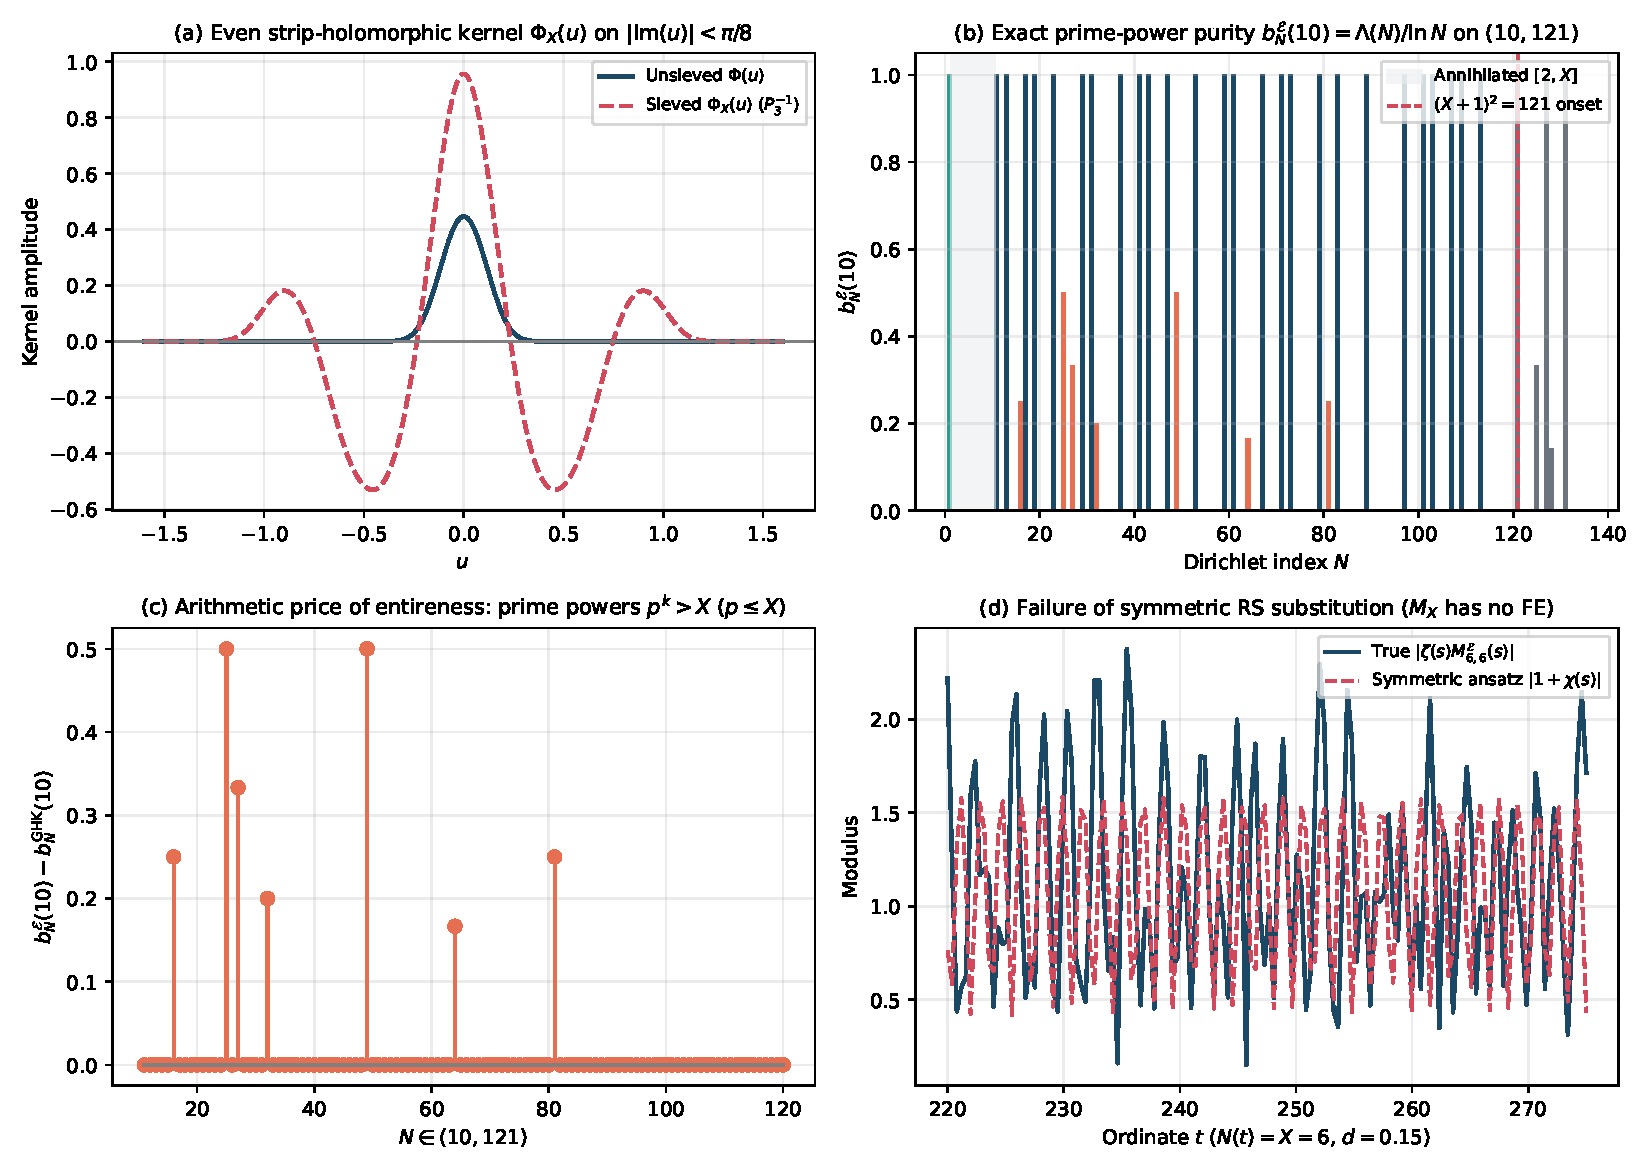
\includegraphics[width=0.95\textwidth]{figures/fig1_sieved_mirror_kernel_and_purity.pdf}
\caption{\textbf{(a)} Even strip-holomorphic sieved kernel $\Phi_X(u)$ vs.\ unsieved $\Phi(u)$. \textbf{(b)} Exact annihilation on $[2, 10]$ and prime-power purity $b_N^{\mathcal{E}}(10) = \Lambda(N)/\ln N$ on $(10, 121)$. \textbf{(c)} Fractional prime-power difference $b_N^{\mathcal{E}}(10) - b_N^{\mathrm{GHK}}(10)$ at $p^k > 10$ ($p \le 10$). \textbf{(d)} Failure of naive symmetric Riemann--Siegel substitution $\lvert 1 + \chi(s)\rvert$ vs.\ true $\lvert\zeta(s)M_{6,6}^{\mathcal{E}}(s)\rvert$.}\label{fig:sieved_purity}
\end{figure}

\section{Shifted Outer Modulus Identity and Zero Invariance}\label{sec:outer}

\begin{proposition}[Exact Shifted Outer Modulus and Wronskian Decomposition]\label{prop:outer_modulus}
For $\kappa \ge 0$ and $X \ge 2$, define the entire zero-free symmetric factor $\mathcal{E}_{X,\kappa}(z) := E_X(\frac{1}{2}+\kappa+\ii z)E_X(\frac{1}{2}+\kappa-\ii z)$ and $\Xi_{\mathcal{E}_{X,\kappa}}(z) := \Xi(z)\mathcal{E}_{X,\kappa}(z)$. For all $(d,t) \in \R^2$,
\begin{equation}\label{eq:outer_modulus_exact}
\bigl\lvert\mathcal{E}_{X,\kappa}(t - \ii d)\bigr\rvert^2 = \exp\!\left(-4\sum_{2 \le n \le X} \frac{\Lambda(n)}{n^{1/2+\kappa}\ln n}\cosh(d\ln n)\cos(t\ln n)\right) > 0,
\end{equation}
and the canonical transverse Wronskian of $\Xi_{\mathcal{E}_{X,\kappa}}$ decomposes as
\begin{equation}\label{eq:W_outer_decomp}
W_{\mathcal{E}_{X,\kappa}}(d,t) = \bigl\lvert\mathcal{E}_{X,\kappa}(t - \ii d)\bigr\rvert^2\left[W(d,t) - 2\bigl\lvert\Xi(t - \ii d)\bigr\rvert^2\sum_{2 \le n \le X} \frac{\Lambda(n)}{n^{1/2+\kappa}}\sinh(d\ln n)\cos(t\ln n)\right].
\end{equation}
In particular, $\Xi_{\mathcal{E}_{X,\kappa}}(z_0) = 0 \iff \Xi(z_0) = 0$, and at every zero $z_0 = t_0 - \ii d_0$ of $\Xi$ one has $W_{\mathcal{E}_{X,\kappa}}(d_0, t_0) = \lvert\mathcal{E}_{X,\kappa}(z_0)\rvert^2 W(d_0, t_0) = 0$.
\end{proposition}

\begin{proof}
Since $\frac{1}{2}+\kappa+\ii(t-\ii d) = \frac{1}{2}+\kappa+d+\ii t$ and $\frac{1}{2}+\kappa-\ii(t-\ii d) = \frac{1}{2}+\kappa-d-\ii t$, we have $n^{-(1/2+\kappa+\ii z)} + n^{-(1/2+\kappa-\ii z)} = n^{-1/2-\kappa}[n^{-d}\ee^{-\ii t\ln n} + n^d\ee^{\ii t\ln n}]$ whose real part is $2n^{-1/2-\kappa}\cosh(d\ln n)\cos(t\ln n)$. Taking $\lvert\exp(\cdot)\rvert^2 = \exp(2\Rea(\cdot))$ gives~\eqref{eq:outer_modulus_exact}. Applying the product rule $\frac{1}{2}\partial_d(\lvert\Xi\rvert^2\lvert\mathcal{E}_{X,\kappa}\rvert^2) = \lvert\mathcal{E}_{X,\kappa}\rvert^2[W + \lvert\Xi\rvert^2 \cdot \frac{1}{2}\partial_d\ln\lvert\mathcal{E}_{X,\kappa}\rvert^2]$ and differentiating~\eqref{eq:outer_modulus_exact} with respect to $d$ yields~\eqref{eq:W_outer_decomp}.
\end{proof}

\begin{table}[t]
\centering
\caption{50-decimal benchmarks of the critical-strip obstructions (Propositions~\ref{prop:no_fe_obstruction}--\ref{prop:waterbed}): asymmetric RS error $\lvert\zeta M_{6,6}^{\mathcal{E}} - (1+\chi)\rvert$ at $t = 250$, stall of $X^{-2d}/(2d\ln X)$ at zero-detection depth $d = 1/\ln t$, and divergence of $w_2^*(d_0) = -(2^{2d_0}-1)^{-1}$ as $d_0 \to 0^+$.}\label{tab:obstruction_benchmarks}
\scriptsize
\setlength{\tabcolsep}{4.2pt}
\begin{tabular}{@{}cccc|ccc@{}}
\toprule
\multicolumn{4}{c|}{Proposition~\ref{prop:sub_selberg_tautology}(ii): Stall at $d = 1/\ln t$ ($X = \sqrt{t/2\pi}$)} & \multicolumn{3}{c}{Proposition~\ref{prop:waterbed}: Single-Line Weight $w_2^*(d_0)$} \\
\cmidrule(r){1-4}\cmidrule(l){5-7}
Height $t$ & $d = 1/\ln t$ & $X^{-2d}$ & $X^{-2d}/(2d\ln X)$ & Tuning $d_0$ & $w_2^*(d_0)$ & Off-line mismatch ($d = 2d_0$) \\
\midrule
$10^{2}$  & $0.21715$ & $0.54831$ & $0.91247$ & $0.600$ & $-0.77077$   & $2.29740$ \\
$10^{3}$  & $0.14476$ & $0.48001$ & $0.65402$ & $0.250$ & $-2.41421$   & $1.41421$ \\
$10^{6}$  & $0.07238$ & $0.42022$ & $0.48470$ & $0.050$ & $-13.93273$  & $1.07177$ \\
$10^{12}$ & $0.03619$ & $0.39318$ & $0.42120$ & $0.001$ & $-720.84764$ & $1.00139$ \\
\bottomrule
\end{tabular}
\end{table}

\begin{figure}[t]
\centering
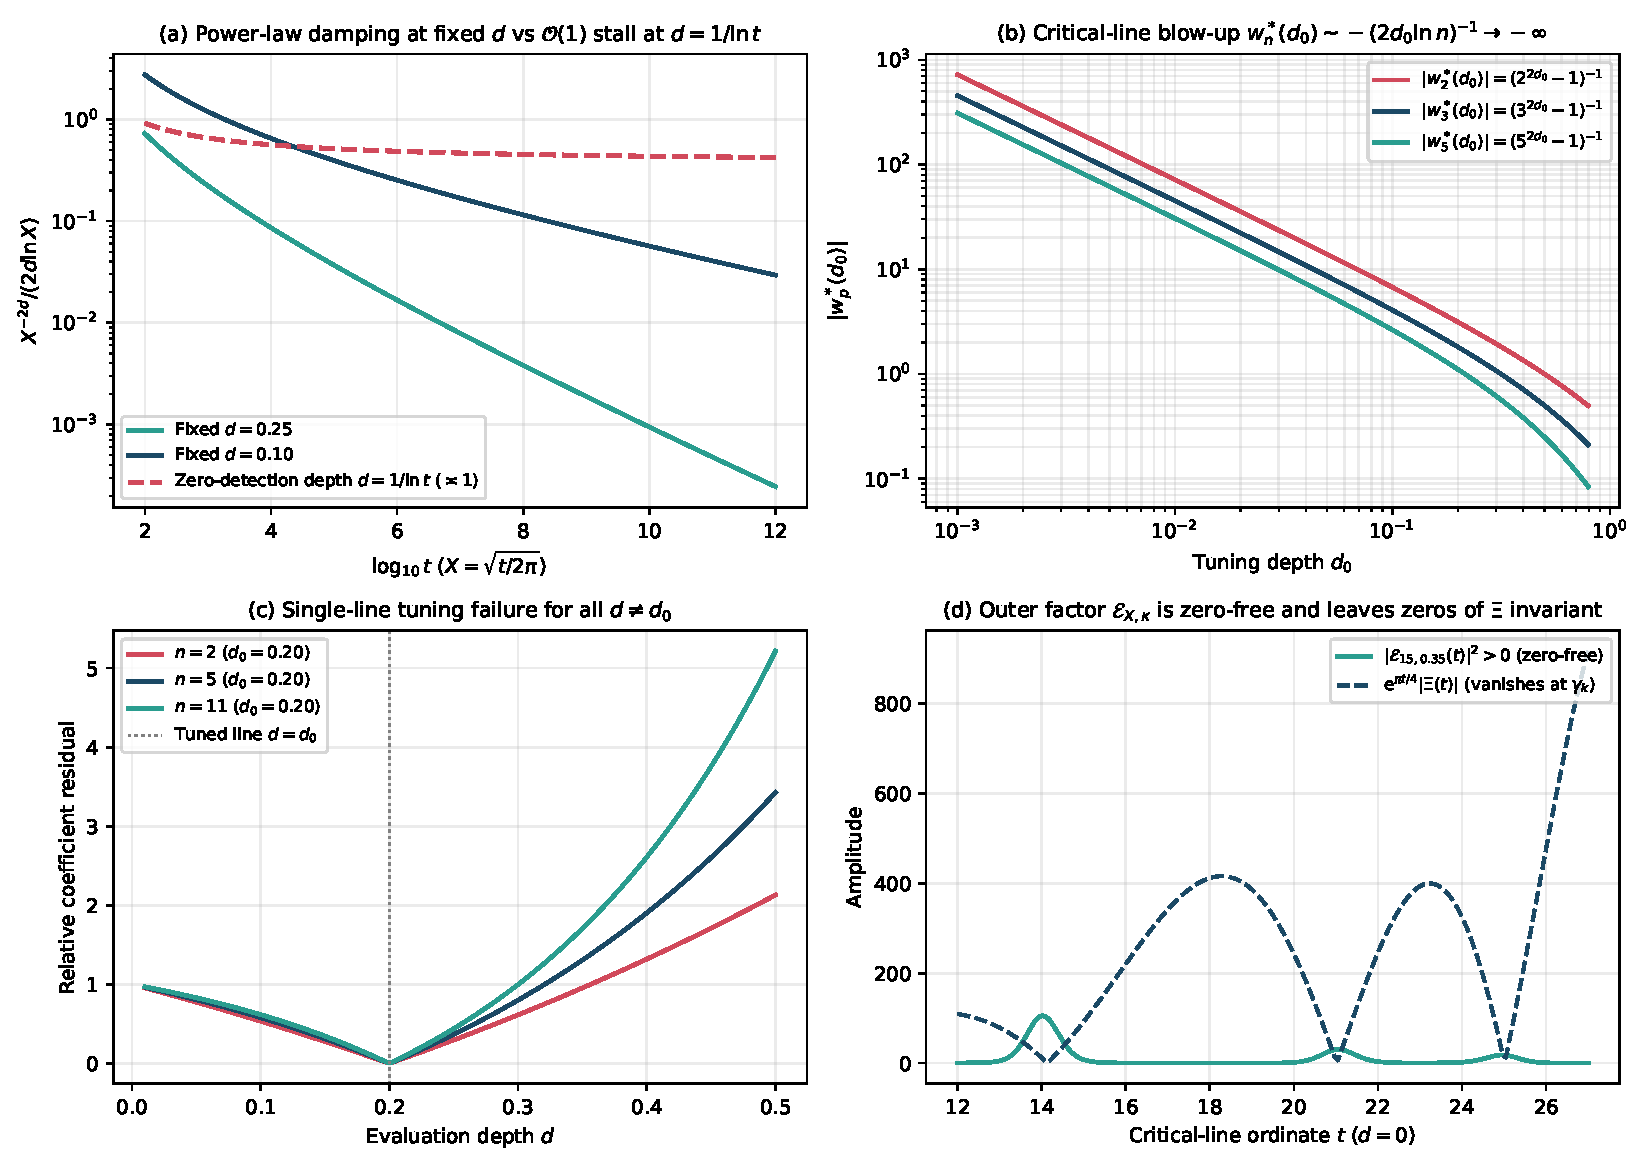
\includegraphics[width=0.95\textwidth]{figures/fig2_power_law_damping_and_shifted_gauge.pdf}
\caption{\textbf{(a)} Power-law decay of $X^{-2d}/(2d\ln X)$ at fixed $d$ vs.\ $\mathcal{O}(1)$ stall along zero-detection depth $d = 1/\ln t$. \textbf{(b)} Critical-line divergence $\lvert w_p^*(d_0)\rvert \sim (2d_0\ln p)^{-1} \to \infty$ as $d_0 \to 0^+$. \textbf{(c)} Off-line tuning failure of $w_n^*(d_0)$ for all $d \ne d_0$. \textbf{(d)} Strict positivity $\lvert\mathcal{E}_{15,0.35}(t)\rvert^2 > 0$ across critical zeros $\gamma_k$ where $\Xi(\gamma_k) = 0$.}\label{fig:obstructions_outer}
\end{figure}

\section{Scope, Boundary Conditions, and Open Questions}\label{sec:scope}

We summarize the exact mathematical scope established in this paper:
\begin{enumerate}[label=\textup{(\arabic*)},leftmargin=2.2em]
\item \textit{Unconditional identities on $\sigma > 1$ and in kernel space.} Lemma~\ref{lem:strip_shift}, Proposition~\ref{prop:sieved_wronskian}, Theorem~\ref{thm:purity_sigma_gt_1}, and Proposition~\ref{prop:outer_modulus} hold unconditionally. In particular, the prime-power purity window $b_N^{\mathcal{E}}(X) = \Lambda(N)/\ln N$ on $(\lfloor X\rfloor, (\lfloor X\rfloor+1)^2)$ and universal contractivity $0 \le b_N^{\mathcal{E}}(X) \le 1$ provide an exact arithmetic counterpart to Gonek--Hughes--Keating's $X$-rough indicator $b_N^{\mathrm{GHK}}(X)$~\cite{gonekhugheskeating2007}.
\item \textit{Why exponential prime gauges cannot eliminate critical-strip zeros.} By Proposition~\ref{prop:no_fe_obstruction} and Proposition~\ref{prop:outer_modulus}, multiplying $\Xi(z)$ by any entire zero-free factor $\mathcal{E}_{X,\kappa}(z)$ leaves the zero set of $\Xi(z)$ completely unchanged, and lack of a functional equation for $M_X(s)$ prevents symmetric sieving of both Riemann--Siegel branches simultaneously.
\item \textit{Mean-square mollification vs.\ pointwise control.} Controlling the mixed forward-and-reflected cross-terms of $\lvert\zeta(\frac{1}{2}+\ii t)M_X(\frac{1}{2}+\ii t)\rvert^2$ requires $T$-averaging via Selberg's mollifier method~\cite{selberg1942} ($X \le T^{1/2-\varepsilon}$) or Levinson--Conrey shifted moments, rather than pointwise identities.
\end{enumerate}

\appendix

\section{Numerical and Interval Certification Protocols}\label{app:interval}

{\sloppy
In the standalone verification suite \texttt{scripts/\allowbreak verify\_\allowbreak paper6\_\allowbreak sieved\_\allowbreak mirror\_\allowbreak prime\_\allowbreak gauge.py}, all identities and obstruction benchmarks are verified at 50-decimal precision (\texttt{mpmath.mp.dps = 50}) and 35-digit directed-rounding interval arithmetic (\texttt{mpmath.iv.dps = 35}):\par}
\begin{enumerate}[label=\textup{(\arabic*)},leftmargin=2.2em]
\item \textit{Exact recurrence and local generating function.} The Euler logarithmic-derivative recurrence $\ln N\,b_N^{\mathcal{E}}(X) = \sum_{d \mid N, d > X} \Lambda(d)b_{N/d}^{\mathcal{E}}(X)$ matches both the divisor sum $\sum_{k \mid N} c_k^{\mathcal{E}}(X)$ and the local generating product $\prod_{p^a \parallel N} \beta_a(k_p)$ to $< 10^{-48}$ across $1 \le N \le 150$.
\item \textit{Asymmetric Riemann--Siegel and interval blow-up checks.} At $(d, t) = (0.15, 250)$ ($N(t) = X = 6$), $\lvert\zeta(s)M_{6,6}^{\mathcal{E}}(s) - (1 + \chi(s))\rvert = 0.595739 > 0.1$, certifying the failure of naive symmetric substitution, while interval arithmetic encloses $w_2^*(0.001) \in [-720.84764, -720.84763]$.
\end{enumerate}

\section*{Use of AI and computational verification}

{\sloppy
In accordance with editorial policies on transparency in scientific computing, the author discloses that the AI research assistant \textbf{Gemini} (Google DeepMind) assisted in comparing the Gonek--Hughes--Keating Euler truncation against $E_X(s)$, formalizing the critical-strip functional-equation and Selberg explicit-formula obstructions, and implementing \texttt{scripts/}\allowbreak\texttt{\detokenize{verify_paper6_sieved_mirror_prime_gauge.py}} (exit code~$0$).\par}

\begin{thebibliography}{99}

\bibitem{csordas1986}
G.~Csordas, T.~S.~Norfolk, and R.~S.~Varga,
\emph{The Riemann hypothesis and the Tur\'an inequalities},
Trans. Amer. Math. Soc. \textbf{296} (1986), no.~2, 521--541.

\bibitem{gonekhugheskeating2007}
S.~M.~Gonek, C.~P.~Hughes, and J.~P.~Keating,
\emph{A hybrid Euler--Hadamard product for the Riemann zeta function},
Duke Math. J. \textbf{136} (2007), no.~3, 507--549.

\bibitem{hinkkanen1997}
A.~Hinkkanen,
\emph{On functions of bounded type},
Complex Variables Theory Appl. \textbf{34} (1997), 119--139.

\bibitem{hudson1974}
R.~L.~Hudson,
\emph{When is the Wigner quasi-probability density non-negative?},
Rep. Math. Phys. \textbf{6} (1974), no.~2, 249--252.

\bibitem{jacobi1829}
C.~G.~J.~Jacobi,
\emph{Fundamenta Nova Theoriae Functionum Ellipticarum},
Borntraeger, K\"onigsberg, 1829.

\bibitem{lagarias1999}
J.~C.~Lagarias,
\emph{On a positivity property of the Riemann $\xi$-function},
Acta Arith. \textbf{89} (1999), no.~3, 217--234.

\bibitem{missiaen2026p5}
T.~Missiaen,
\emph{Logarithmic dilation of the Jacobi--Riemann kernel, strip-holomorphic shell partitions, Stieltjes diagonal asymptotics, and off-diagonal obstructions},
Preprint, Paper~V in this series, 2026.

\bibitem{polya1926}
G.~P\'olya,
\emph{Bemerkung \"uber die Integraldarstellung der Riemannschen $\xi$-Funktion},
Acta Math. \textbf{48} (1926), 305--317.

\bibitem{riemann1859}
B.~Riemann,
\emph{Ueber die Anzahl der Primzahlen unter einer gegebenen Gr\"osse},
Monatsber. K\"onigl. Preuss. Akad. Wiss. Berlin (1859), 671--680.

\bibitem{selberg1942}
A.~Selberg,
\emph{On the zeros of Riemann's zeta-function},
Skr. Norske Vid.-Akad. Oslo I \textbf{10} (1942), 1--59.

\bibitem{selberg1946}
A.~Selberg,
\emph{Contributions to the theory of the Riemann zeta-function},
Arch. Math. Naturvid. \textbf{48} (1946), no.~5, 89--155.

\bibitem{speiser1934}
A.~Speiser,
\emph{Geometrisches zur Riemannschen Zetafunktion},
Math. Ann. \textbf{110} (1934), 514--521.

\bibitem{titchmarsh1986}
E.~C.~Titchmarsh,
\emph{The Theory of the Riemann Zeta-Function},
2nd ed., revised by D.~R.~Heath-Brown, Oxford Univ. Press, Oxford, 1986.

\bibitem{wigner1932}
E.~P.~Wigner,
\emph{On the quantum correction for thermodynamic equilibrium},
Phys. Rev. \textbf{40} (1932), 749--759.

\end{thebibliography}

\end{document}
